% Compile twice with XeLaTeX from this directory.
\documentclass[a4paper,11pt]{article}
\usepackage[margin=20mm]{geometry}
\usepackage{fontspec}
\defaultfontfeatures{Ligatures=TeX}
\IfFileExists{/mnt/c/Windows/Fonts/times.ttf}{%
  \setmainfont[Path=/mnt/c/Windows/Fonts/,BoldFont=timesbd.ttf,
    ItalicFont=timesi.ttf,BoldItalicFont=timesbi.ttf]{times.ttf}
}{\setmainfont{Times New Roman}}
\usepackage{amsmath,unicode-math}
\setmathfont{TeX Gyre Termes Math}
\usepackage{graphicx,booktabs,tabularx,array,caption,titlesec}
\usepackage[hidelinks]{hyperref}
\graphicspath{{figures/}}
\captionsetup{font=small,labelfont=bf,justification=raggedright,singlelinecheck=false}
\titleformat{\section}{\large\bfseries}{\thesection.}{.5em}{}
\titleformat{\subsection}{\normalsize\bfseries}{\thesubsection}{.5em}{}
\titlespacing*{\section}{0pt}{8pt}{8pt}
\titlespacing*{\subsection}{0pt}{8pt}{7pt}
\setlength{\parindent}{0pt}
\setlength{\parskip}{6pt}
\setlength{\emergencystretch}{2em}
\renewcommand{\arraystretch}{1.15}
\newcommand{\Msun}{M_{\odot}}
\newcommand{\vtmean}{\langle v_t\rangle}
\newcolumntype{Y}{>{\raggedright\arraybackslash}X}
\hypersetup{pdftitle={Rotation Curves: Configuration, Evolution and Results}}
\begin{document}
{\LARGE\bfseries Rotation Curves\par}
\section{Configuration}
The eight experiments combine two halo mass labels,
$M=10^9$ and $10^{10}\,\Msun$, two initial fractional speed scatters,
$f=0$ and $0.1$, and two potential histories: continuously evolving or
held fixed after $t_f=1\,\mathrm{Gyr}$. Each run contains 600,000
non-self-gravitating stellar test particles in an FDM halo with
$m_a=10^{-22}\,\mathrm{eV}/c^2$ and halo seed 0.

\begin{center}
\begin{tabular}{@{}cccc@{}}
\toprule
Run & $M\;(\Msun)$ & $f$ & Potential after 1 Gyr\\
\midrule
E1 & $10^9$ & 0 & Evolving\\
E2 & $10^9$ & 0.1 & Evolving\\
E3 & $10^{10}$ & 0 & Evolving\\
E4 & $10^{10}$ & 0.1 & Evolving\\
F1 & $10^9$ & 0 & Frozen at 1 Gyr\\
F2 & $10^9$ & 0.1 & Frozen at 1 Gyr\\
F3 & $10^{10}$ & 0 & Frozen at 1 Gyr\\
F4 & $10^{10}$ & 0.1 & Frozen at 1 Gyr\\
\bottomrule
\end{tabular}
\end{center}

\textbf{Initial positions and velocities.}
The initial radii span $0<r<30\,\mathrm{kpc}$, with equal particle counts
in 600 shells of width $0.05\,\mathrm{kpc}$. Sampling is uniform in volume
within each shell and isotropic in angle. The velocity direction is
random in the plane perpendicular to the position vector; it does not
impose a common sense of rotation about $z$. Its magnitude is
\begin{equation}
 \mathbf v_0=\hat{\mathbf e}_t\,v_{c,0}(r_0)\max(1+\epsilon,0),
 \qquad \hat{\mathbf e}_t\cdot\mathbf r_0=0,
 \qquad \epsilon\sim\mathcal N(0,f^2),
\end{equation}
where $v_{c,0}$ is calculated from the smooth modal baseline used at
$t=0$. Thus $f=0.1$ changes the speed magnitude by a Gaussian scatter
of 10\%; the initial radial velocity is zero in both cases.

\textbf{Halo and output settings.}
The archived potentials use a soliton plus Hernquist-envelope halo,
represented by an eigenmode superposition and an AGAMA multipole
expansion with $l_{\max}=20$. Potential snapshots have a 0.1 Gyr cadence and are
linearly interpolated for the orbit calculation. The trajectories have
111 stored frames; this report selects frames 0, 10, 50 and 110,
labelled $t=0,1,5,11\,\mathrm{Gyr}$ in the MP4s. All velocity profiles
use the full particle population, 90 bins over 0--30 kpc
($\Delta r=\Delta R=1/3\,\mathrm{kpc}$), and at least 40 particles per bin.

\textbf{Coordinate and time conventions.}
The existing evolving MP4s use stored tracer-centered positions with
unshifted velocities; their no-scatter time labels are nominal because
the legacy files do not store an explicit time vector. The frozen runs
use unshifted halo-centered positions and velocities, with explicit
0.1 Gyr output times. The figures retain these MP4 conventions.

\clearpage
\section{Evolution and velocity definitions}
During $0\leq t\leq1\,\mathrm{Gyr}$, the fluctuating density is introduced
by a linear ramp from the smooth modal density $\bar\rho$:
\begin{equation}
 \rho_{\rm drive}(\mathbf x,t)=[1-s(t)]\bar\rho(r)
                  +s(t)\rho_{\rm FDM}(\mathbf x,t),
 \qquad s(t)=\min\!\left(\frac{t}{1\,\mathrm{Gyr}},1\right).
\end{equation}
The potential is constructed from this density. In E1--E4 the mode
phases and potential continue to evolve after the ramp. In F1--F4,
the full nonspherical potential of snapshot 010 is held fixed:
\begin{equation}
 \Phi_F(\mathbf x,t)=
 \begin{cases}
  \Phi_E(\mathbf x,t),&t\leq1\,\mathrm{Gyr},\\
  \Phi_E(\mathbf x,1\,\mathrm{Gyr}),&t>1\,\mathrm{Gyr}.
 \end{cases}
\end{equation}
The stellar orbits continue to 11 Gyr in both histories, obeying
$\ddot{\mathbf x}=-\nabla\Phi(\mathbf x,t)$.

\textbf{Particle tangential speed.}
For each stored phase-space point, let $r=|\mathbf x|$ and
$R=\sqrt{x^2+y^2}$. The speed plotted for individual particles in the
MP4s, and averaged for the main profile, is
\begin{equation}
 v_t=\frac{|\mathbf x\times\mathbf v|}{r}
     =\sqrt{|\mathbf v|^2-
       \left(\frac{\mathbf x\cdot\mathbf v}{r}\right)^2},
 \qquad
 \vtmean_j=\frac1{N_j}\sum_{i\in\mathcal S_j}v_{t,i},
 \qquad \mathcal S_j=\{i:r_i\in[r_j^-,r_j^+)\}.
 \label{eq:vt}
\end{equation}
This is the magnitude of the velocity perpendicular to the radius
vector, not the total three-dimensional speed or a signed rotation speed.
The blue solid line in all eight figures shows $\vtmean(r,t)$.

\textbf{Azimuthal speed about $z$.}
The green solid line in all eight figures shows the mean absolute
azimuthal speed, calculated from the same stored phase-space frames:
\begin{equation}
 v_\phi=\frac{xv_y-yv_x}{R},\qquad
 \langle|v_\phi|\rangle_j=\frac1{N_j^R}
       \sum_{i\in\mathcal C_j}|v_{\phi,i}|,
 \qquad \mathcal C_j=\{i:R_i\in[R_j^-,R_j^+)\}.
 \label{eq:phi}
\end{equation}
Its horizontal coordinate is cylindrical $R$; the other curves use
spherical $r$. The absolute value prevents cancellation of oppositely
directed motions. The same statistic and plotting convention are used
for the evolving and frozen halos.

\textbf{Circular-speed reference and shaded bands.}
The red dashed line in all eight figures shows
\begin{equation}
 v_c(r,t)=\sqrt{\frac{G M_{\rm halo}(<r,t)}{r}},\qquad
 M_{\rm halo}(<r,t)=\int_{|\mathbf x|<r}\rho_{\rm drive}(\mathbf x,t)\,d^3x.
 \label{eq:vc}
\end{equation}
This spherical enclosed-mass reference uses the stored potential;
$M$ in the run table is a model label, not a replacement for
$M_{\rm halo}(<r,t)$. The frozen reference stays constant for $t\geq1$ Gyr.
Each band spans the corresponding mean plus or minus the within-bin
particle standard deviation:
\begin{equation}
 \sigma_q^2=\frac1N\sum_i(q_i-\langle q\rangle)^2,
 \qquad q=v_t\ \text{or}\ |v_\phi|.
\end{equation}
Blue and green bands belong to their matching lines in all eight
figures. These are speed dispersions, not errors on the mean.
Figures 1--8 use the stored frames corresponding to the four selected
MP4 epochs, ordered left-to-right and then top-to-bottom.

\clearpage
\section{Results}
The MP4 animations can be viewed in the accompanying \texttt{mp4/}
directory (\texttt{report/mp4/} in the project). A link to the corresponding
animation is provided below each figure.

Each figure represents one complete evolution. The four panels are
$t=0,1,5,11\,\mathrm{Gyr}$; axis limits are shared within each figure.
\subsection{\texorpdfstring{E1: $M=10^{9}\,\Msun$, $f=0$, evolving halo}{E1: M=1e9 solar masses, f=0, evolving halo}}
\begin{figure}[!ht]
\centering
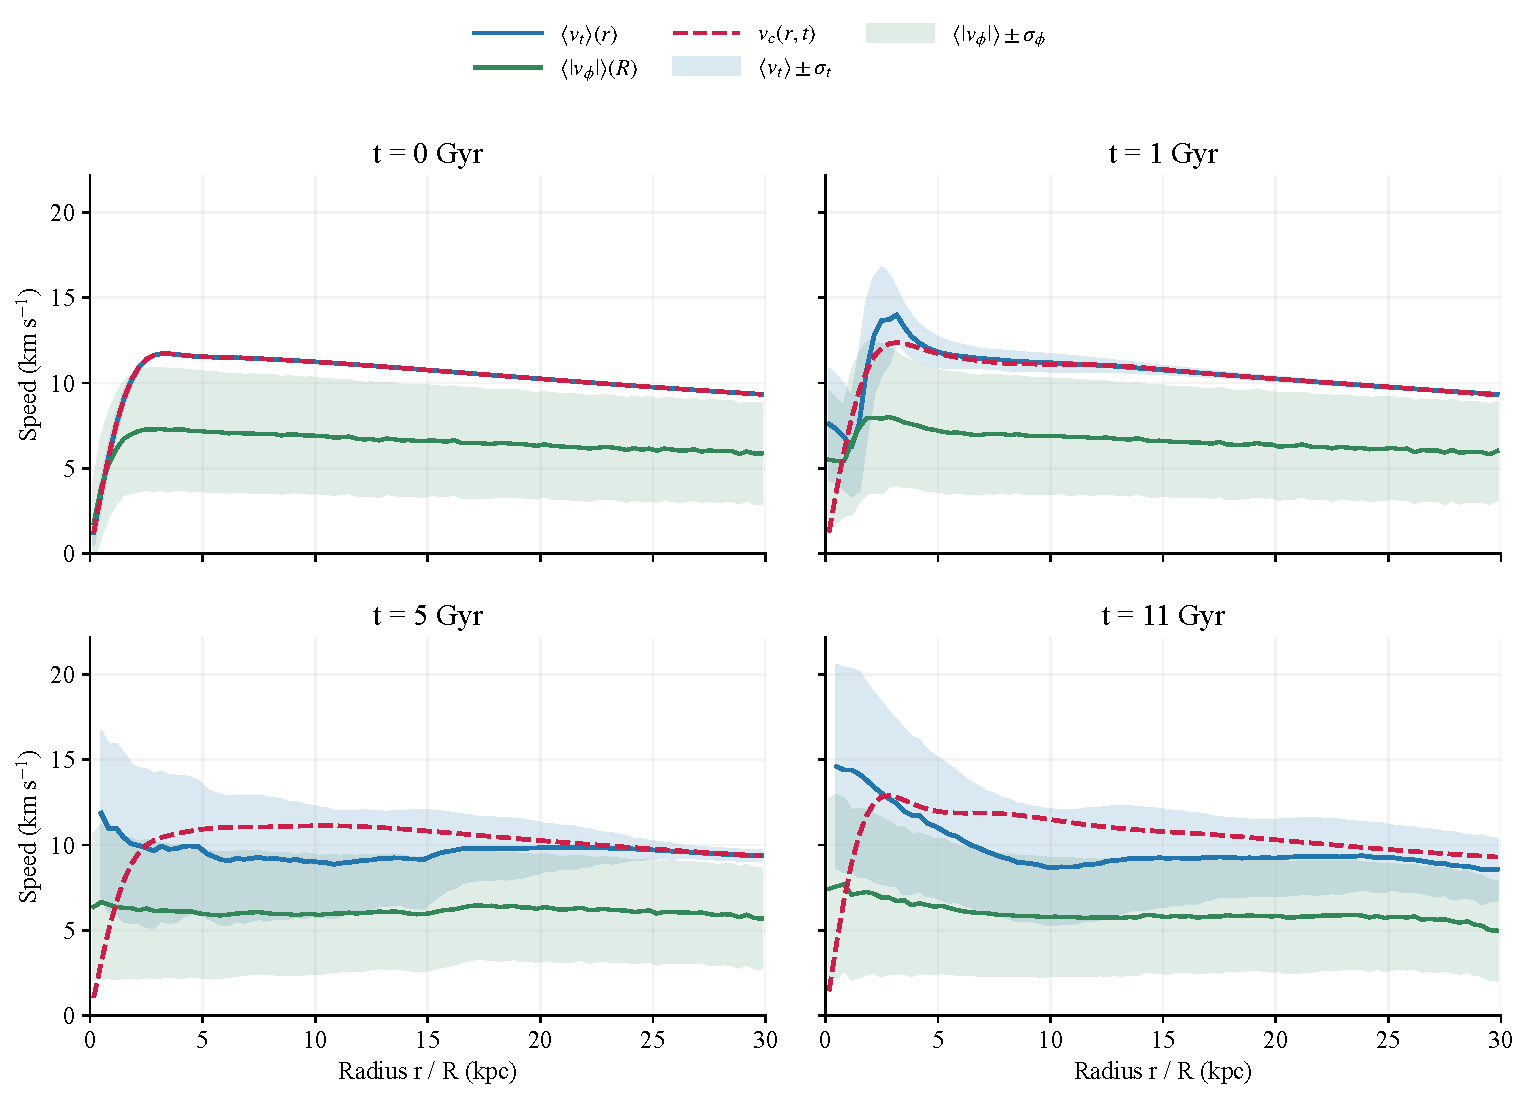
\includegraphics[width=\linewidth]{rotation_E1_M1e9_f0.0_four_epochs.pdf}
\caption{E1. Blue solid: $\vtmean(r,t)$. Green solid: $\langle|v_\phi|\rangle(R,t)$. Red dashed: $v_c(r,t)$. Blue and green bands: the corresponding mean $\pm1\sigma$. The green curve uses cylindrical $R$; the others use spherical $r$.}\label{fig:E1}
\end{figure}
\textbf{Animation:} \href{run:mp4/E1_M1e9_f0.0_evolving.mp4}{View the E1 MP4 animation.}

The initially narrow tangential-speed profile follows $v_c$. By 5 Gyr the distribution has broadened and the mean lies below the reference over much of the intermediate-radius range. This offset remains at 11 Gyr; the central bins instead show a rising mean and a large dispersion. The green curve is lower because it measures only the absolute azimuthal component, with a different radial binning.

For $B(t)=\operatorname{median}_{5\leq r/\mathrm{kpc}\leq20}[\vtmean/v_c]$, the four panels give $1.000$, $1.001$, $0.840$, $0.846$, respectively.
At 11 Gyr and $r=10\,\mathrm{kpc}$, $\vtmean=8.69\,\mathrm{km\,s^{-1}}$ and $v_c=11.49\,\mathrm{km\,s^{-1}}$.

\clearpage
\subsection{\texorpdfstring{E2: $M=10^{9}\,\Msun$, $f=0.1$, evolving halo}{E2: M=1e9 solar masses, f=0.1, evolving halo}}
\begin{figure}[!ht]
\centering
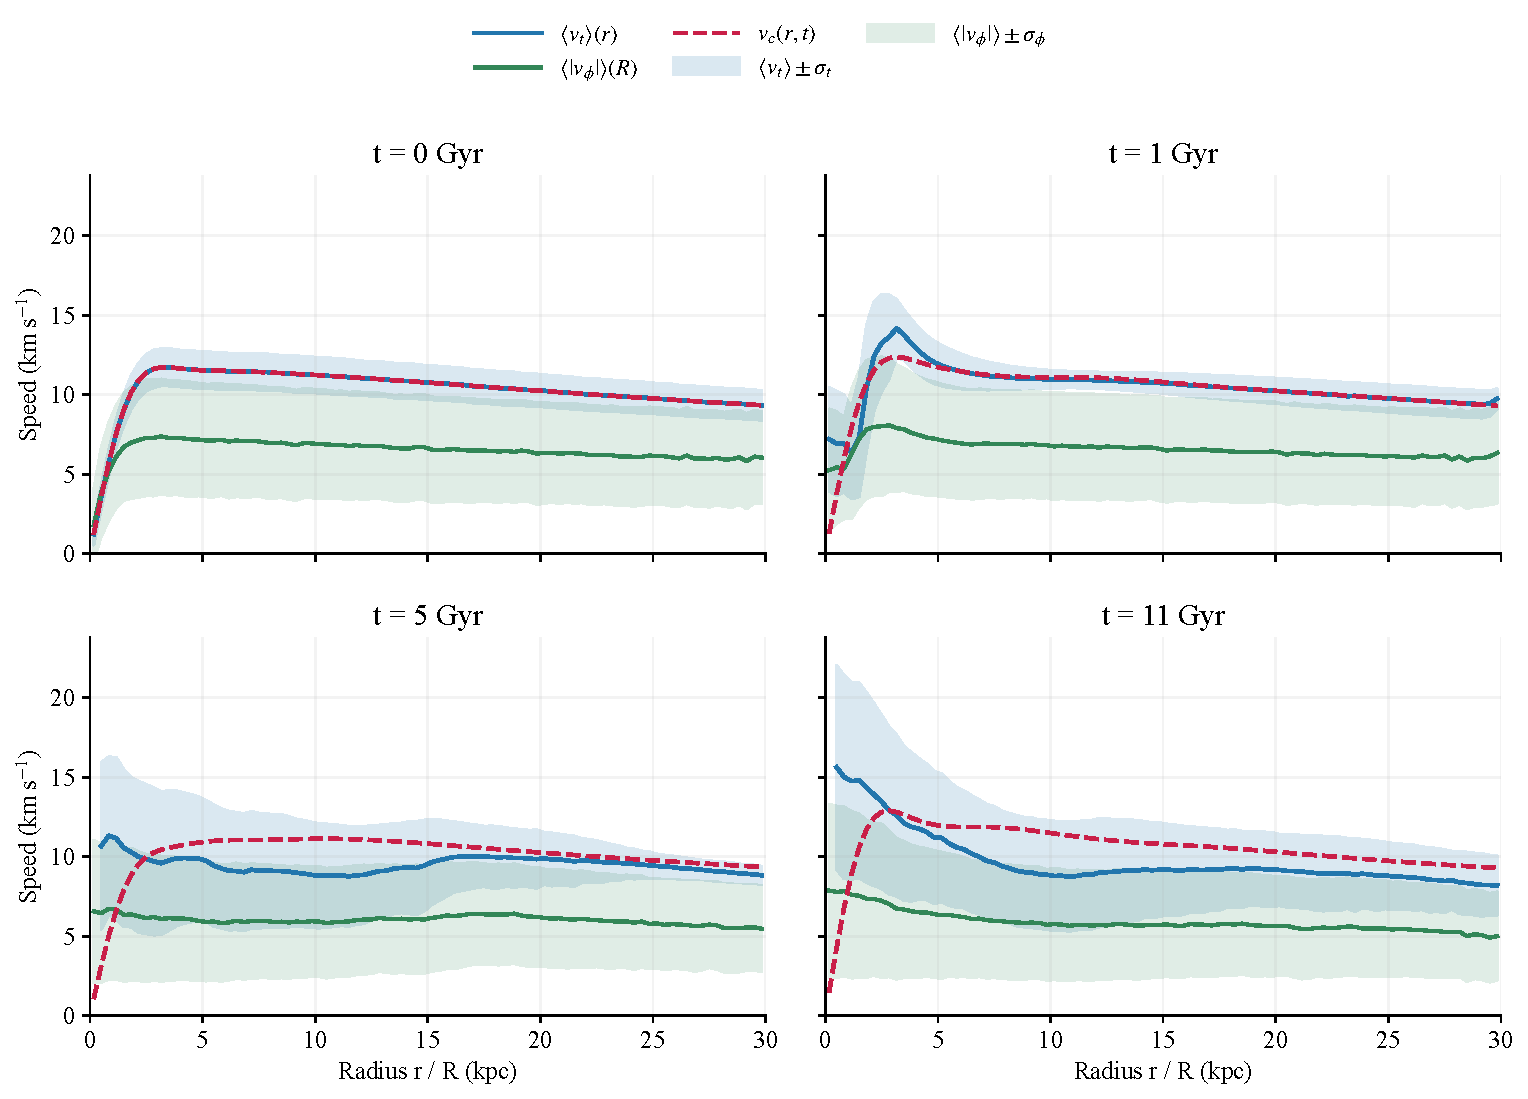
\includegraphics[width=\linewidth]{rotation_E2_M1e9_f0.1_four_epochs.pdf}
\caption{E2. Blue solid: $\vtmean(r,t)$. Green solid: $\langle|v_\phi|\rangle(R,t)$. Red dashed: $v_c(r,t)$. Blue and green bands: the corresponding mean $\pm1\sigma$. The green curve uses cylindrical $R$; the others use spherical $r$.}\label{fig:E2}
\end{figure}
\textbf{Animation:} \href{run:mp4/E2_M1e9_f0.1_evolving.mp4}{View the E2 MP4 animation.}

The imposed 10\% scatter is visible in the initial blue band. After the ramp, the subsequent evolution develops an intermediate-radius deficit and a broad inner distribution similar to E1. The late deficit therefore also occurs when the particles begin with a finite speed dispersion; the change is not confined to the initially cold case.

For $B(t)=\operatorname{median}_{5\leq r/\mathrm{kpc}\leq20}[\vtmean/v_c]$, the four panels give $1.000$, $0.993$, $0.840$, $0.844$, respectively.
At 11 Gyr and $r=10\,\mathrm{kpc}$, $\vtmean=8.83\,\mathrm{km\,s^{-1}}$ and $v_c=11.49\,\mathrm{km\,s^{-1}}$.

\clearpage
\subsection{\texorpdfstring{E3: $M=10^{10}\,\Msun$, $f=0$, evolving halo}{E3: M=1e10 solar masses, f=0, evolving halo}}
\begin{figure}[!ht]
\centering
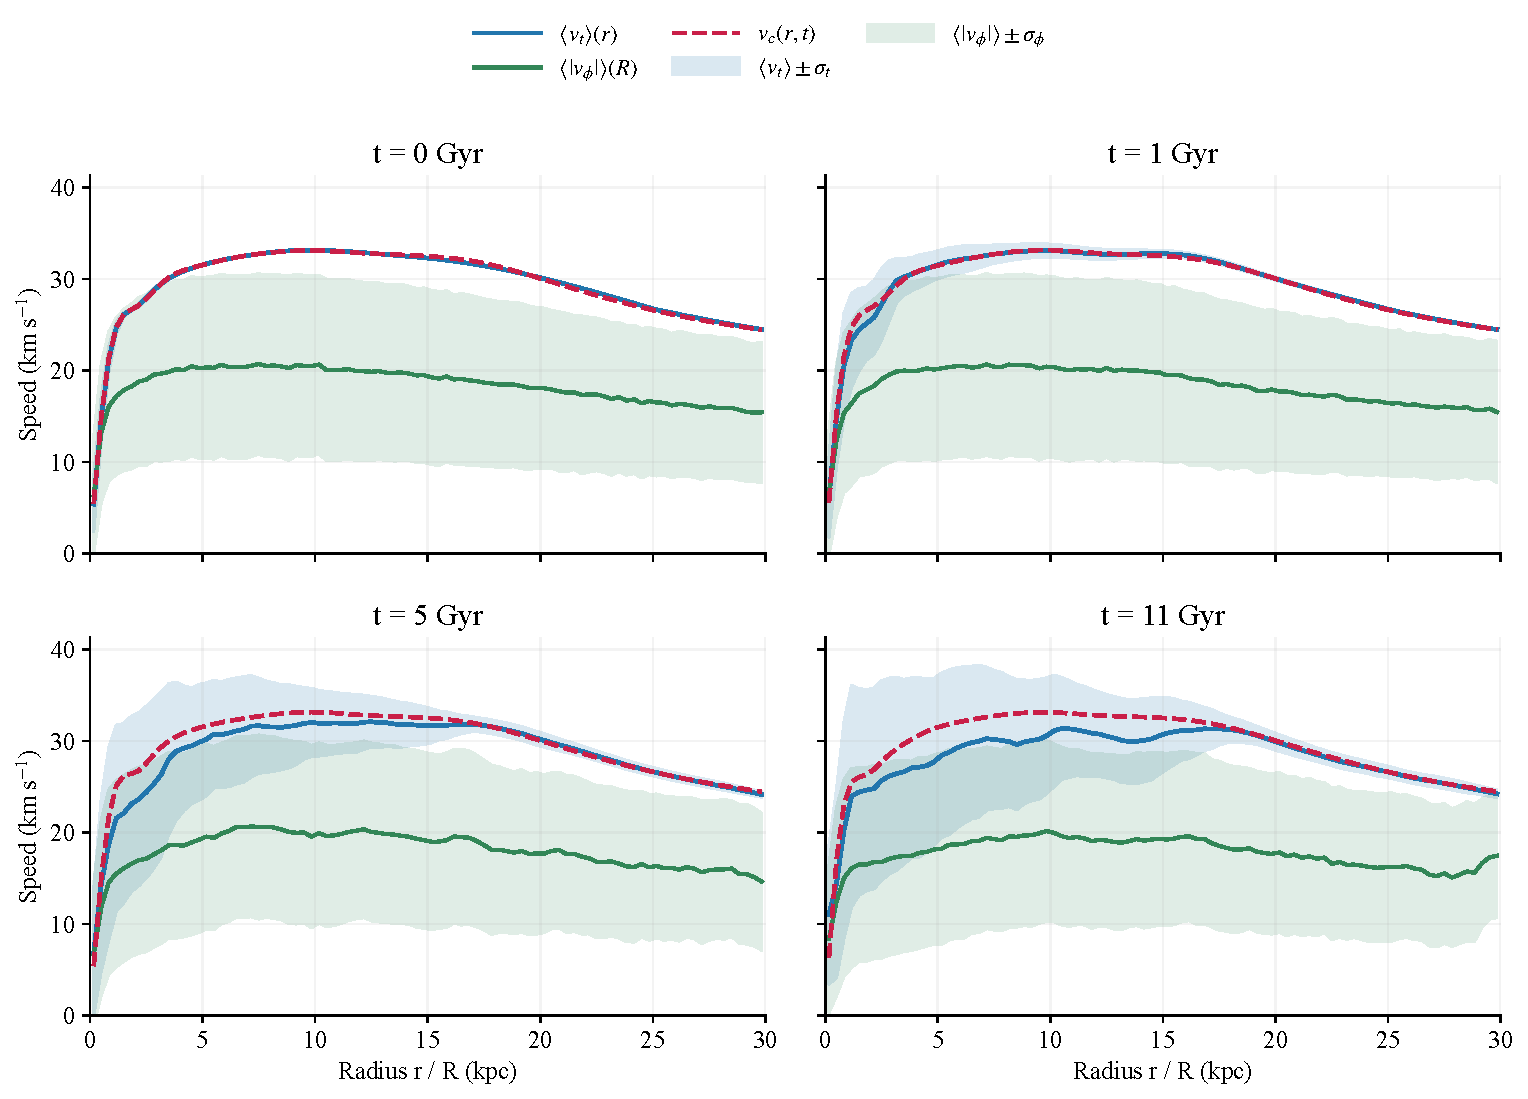
\includegraphics[width=\linewidth]{rotation_E3_M1e10_f0.0_four_epochs.pdf}
\caption{E3. Blue solid: $\vtmean(r,t)$. Green solid: $\langle|v_\phi|\rangle(R,t)$. Red dashed: $v_c(r,t)$. Blue and green bands: the corresponding mean $\pm1\sigma$. The green curve uses cylindrical $R$; the others use spherical $r$.}\label{fig:E3}
\end{figure}
\textbf{Animation:} \href{run:mp4/E3_M1e10_f0.0_evolving.mp4}{View the E3 MP4 animation.}

The higher-mass halo has a larger circular-speed scale. The initial mean again follows the reference, while the late profiles develop a smaller intermediate-radius deficit than in E1. The difference between 5 and 11 Gyr shows that the late-time profile is still evolving; an offset from the reference does not by itself demonstrate a stationary stellar distribution.

For $B(t)=\operatorname{median}_{5\leq r/\mathrm{kpc}\leq20}[\vtmean/v_c]$, the four panels give $1.000$, $1.000$, $0.974$, $0.938$, respectively.
At 11 Gyr and $r=10\,\mathrm{kpc}$, $\vtmean=30.85\,\mathrm{km\,s^{-1}}$ and $v_c=33.13\,\mathrm{km\,s^{-1}}$.

\clearpage
\subsection{\texorpdfstring{E4: $M=10^{10}\,\Msun$, $f=0.1$, evolving halo}{E4: M=1e10 solar masses, f=0.1, evolving halo}}
\begin{figure}[!ht]
\centering
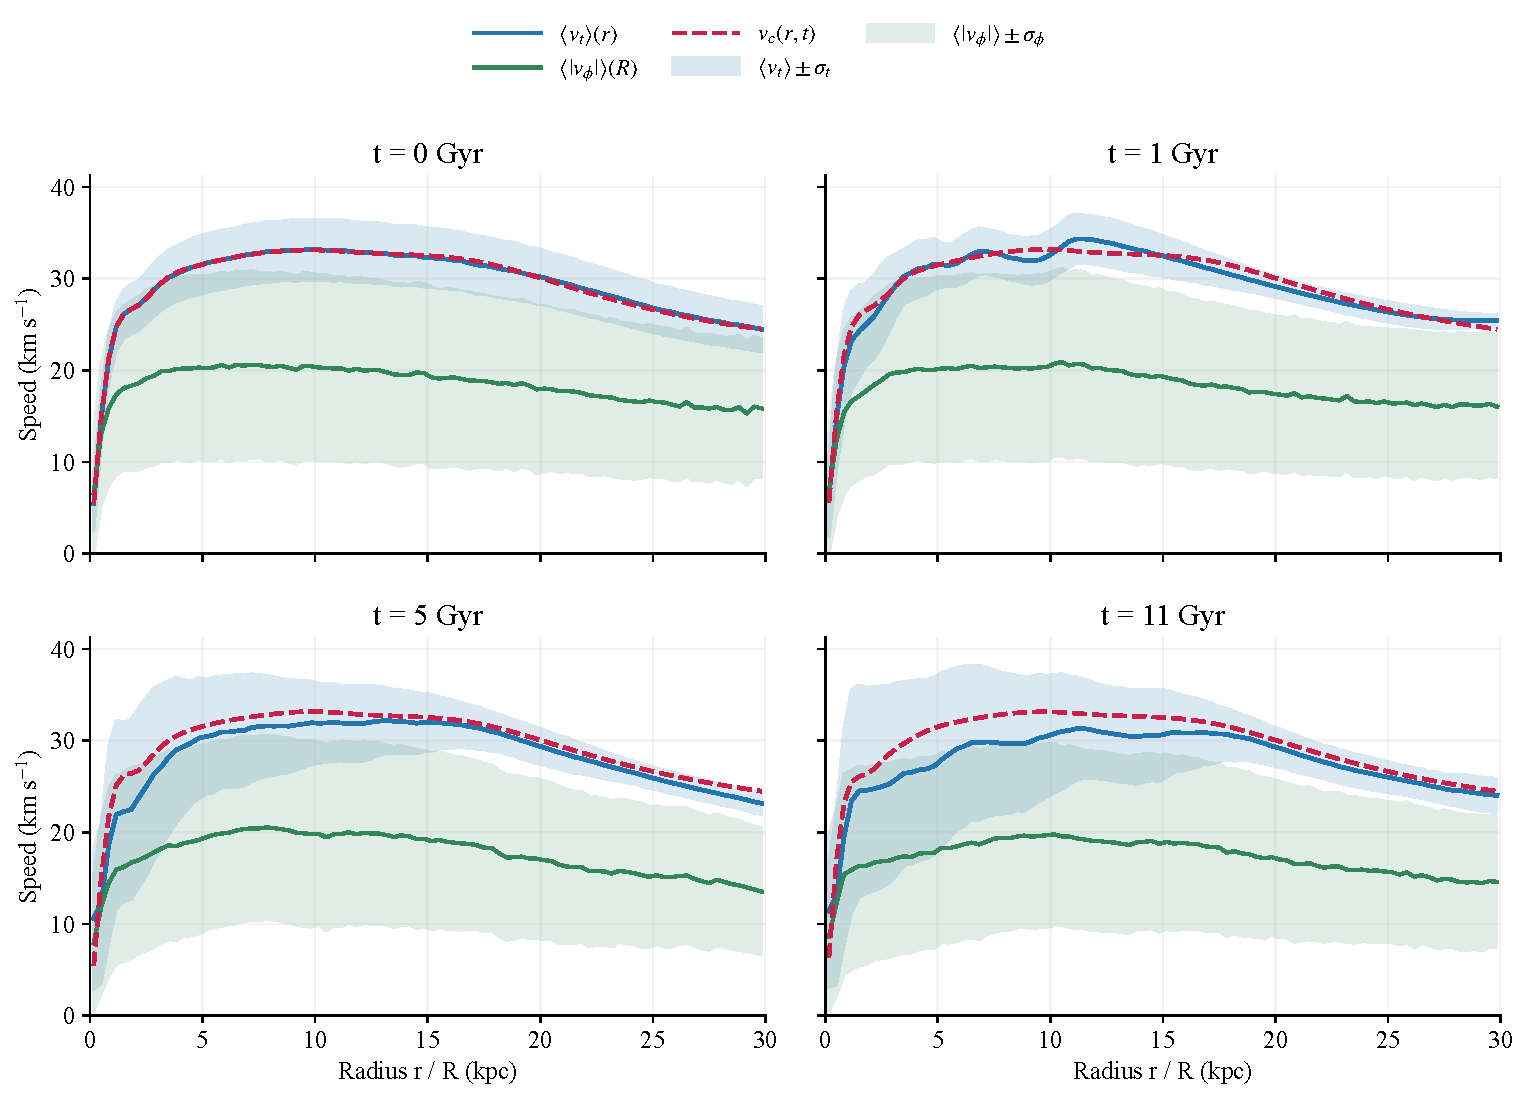
\includegraphics[width=\linewidth]{rotation_E4_M1e10_f0.1_four_epochs.pdf}
\caption{E4. Blue solid: $\vtmean(r,t)$. Green solid: $\langle|v_\phi|\rangle(R,t)$. Red dashed: $v_c(r,t)$. Blue and green bands: the corresponding mean $\pm1\sigma$. The green curve uses cylindrical $R$; the others use spherical $r$.}\label{fig:E4}
\end{figure}
\textbf{Animation:} \href{run:mp4/E4_M1e10_f0.1_evolving.mp4}{View the E4 MP4 animation.}

The initial 10\% scatter broadens the stellar-speed distribution while leaving its mean close to the circular-speed reference. At late times the intermediate-radius mean is close to that in E3, with a smaller deficit than in the lower-mass evolving runs. The initial scatter changes the distribution width more visibly than the final median speed ratio.

For $B(t)=\operatorname{median}_{5\leq r/\mathrm{kpc}\leq20}[\vtmean/v_c]$, the four panels give $1.000$, $0.992$, $0.977$, $0.939$, respectively.
At 11 Gyr and $r=10\,\mathrm{kpc}$, $\vtmean=30.60\,\mathrm{km\,s^{-1}}$ and $v_c=33.13\,\mathrm{km\,s^{-1}}$.

\clearpage
\subsection{\texorpdfstring{F1: $M=10^{9}\,\Msun$, $f=0$, frozen at 1 Gyr}{F1: M=1e9 solar masses, f=0, frozen at 1 Gyr}}
\begin{figure}[!ht]
\centering
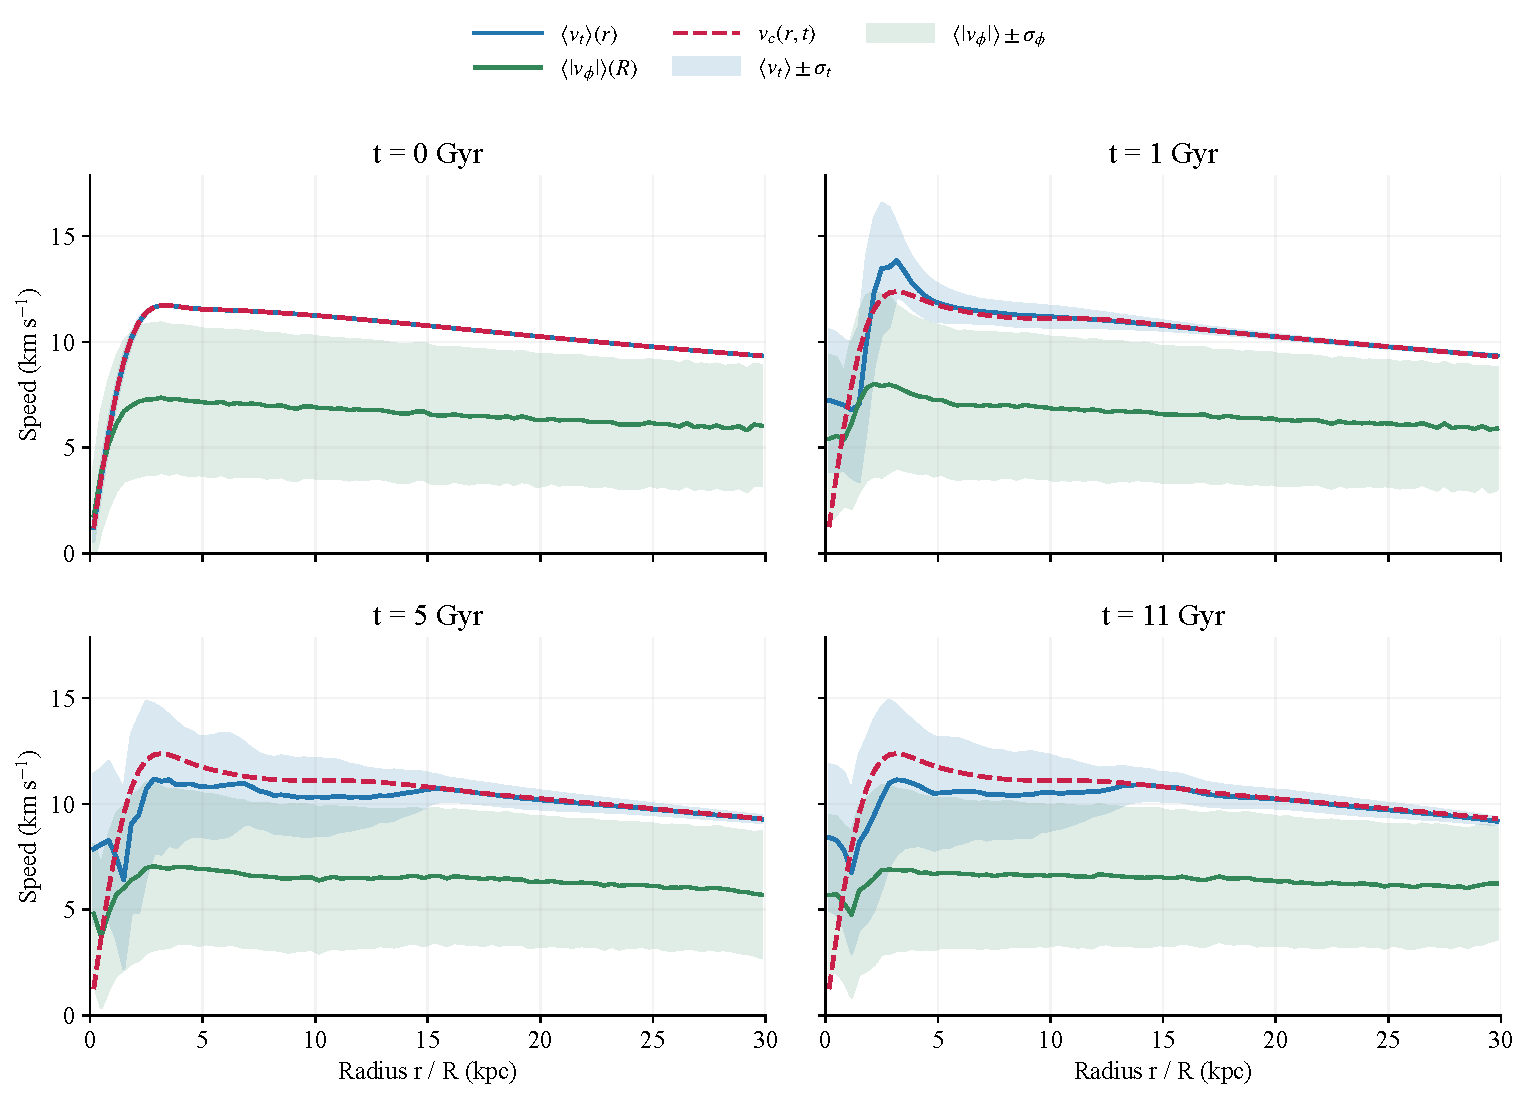
\includegraphics[width=\linewidth]{rotation_F1_M1e9_f0.0_four_epochs.pdf}
\caption{F1. Blue solid: $\vtmean(r,t)$. Green solid: $\langle|v_\phi|\rangle(R,t)$. Red dashed: $v_c(r,t)$. Blue and green bands: the corresponding mean $\pm1\sigma$. The green curve uses cylindrical $R$; the others use spherical $r$. The potential and red dashed reference are held fixed from 1 Gyr onward.}\label{fig:F1}
\end{figure}
\textbf{Animation:} \href{run:mp4/F1_M1e9_f0.0_frozen1Gyr.mp4}{View the F1 MP4 animation.}

The 0--1 Gyr history introduces the fluctuating halo, after which the reference curve is identical in the 1, 5 and 11 Gyr panels. The stellar profile continues to change in this fixed nonspherical field. By 11 Gyr the intermediate-radius mean is closer to the reference than in E1, while an inner speed deficit and a broad central distribution remain.

For $B(t)=\operatorname{median}_{5\leq r/\mathrm{kpc}\leq20}[\vtmean/v_c]$, the four panels give $1.000$, $1.001$, $0.953$, $0.965$, respectively.
At 11 Gyr and $r=10\,\mathrm{kpc}$, $\vtmean=10.52\,\mathrm{km\,s^{-1}}$ and $v_c=11.11\,\mathrm{km\,s^{-1}}$.

\clearpage
\subsection{\texorpdfstring{F2: $M=10^{9}\,\Msun$, $f=0.1$, frozen at 1 Gyr}{F2: M=1e9 solar masses, f=0.1, frozen at 1 Gyr}}
\begin{figure}[!ht]
\centering
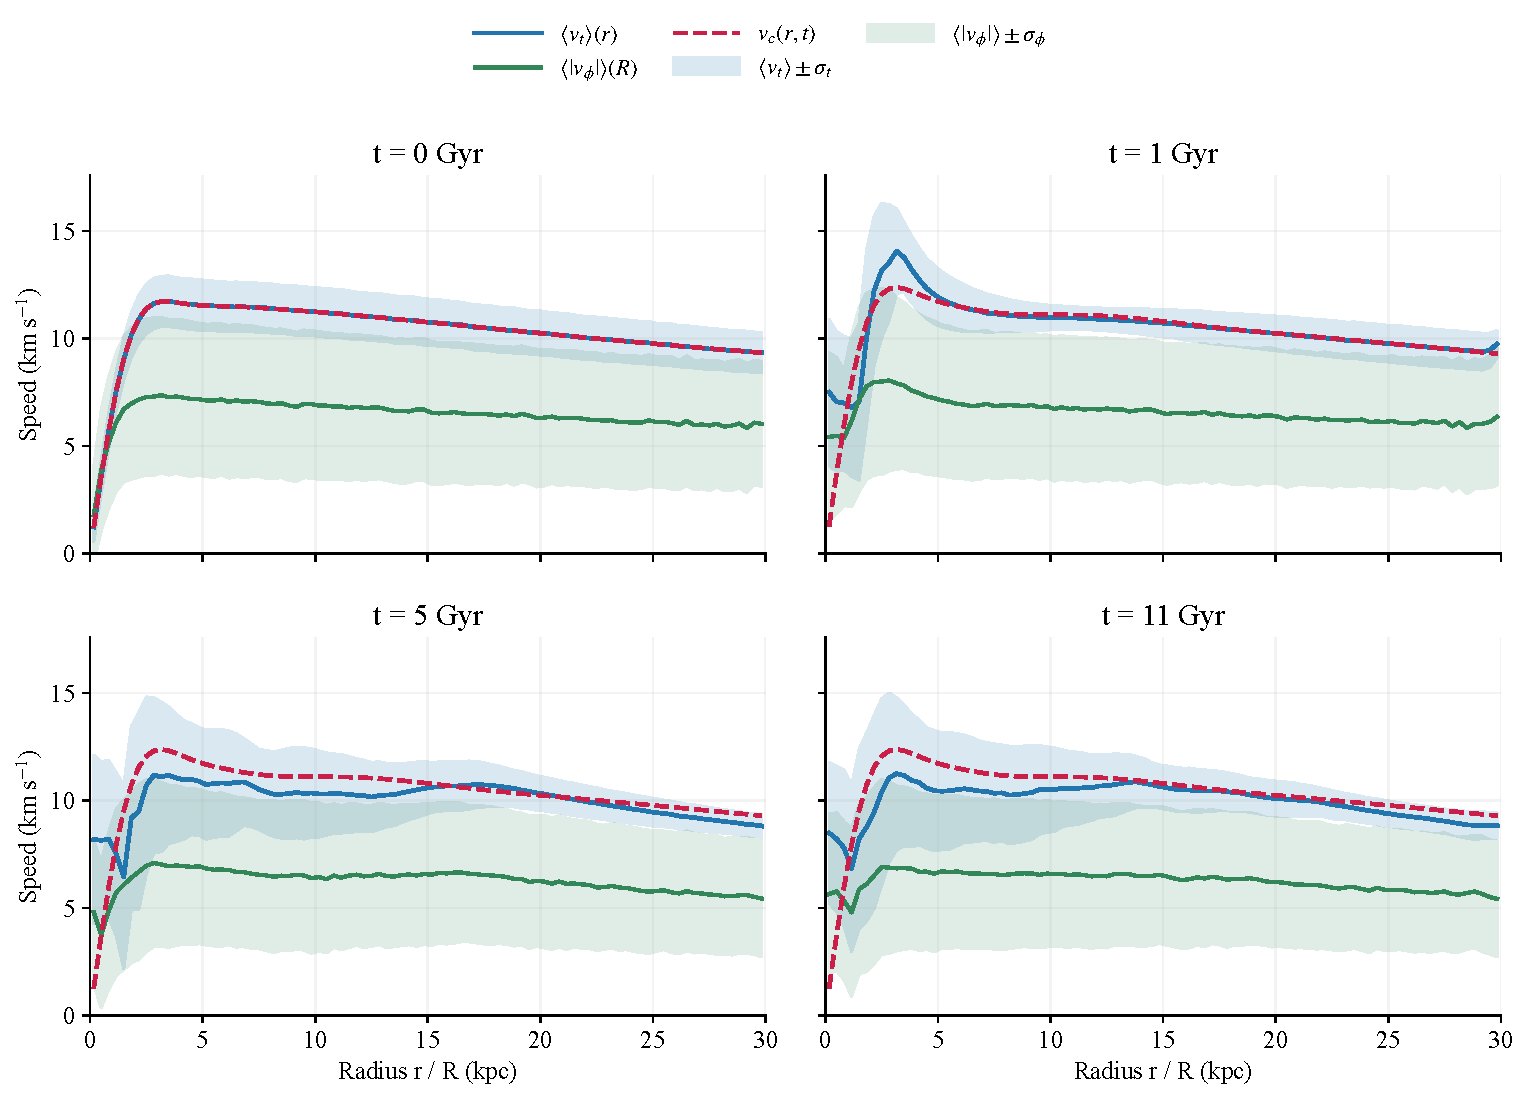
\includegraphics[width=\linewidth]{rotation_F2_M1e9_f0.1_four_epochs.pdf}
\caption{F2. Blue solid: $\vtmean(r,t)$. Green solid: $\langle|v_\phi|\rangle(R,t)$. Red dashed: $v_c(r,t)$. Blue and green bands: the corresponding mean $\pm1\sigma$. The green curve uses cylindrical $R$; the others use spherical $r$. The potential and red dashed reference are held fixed from 1 Gyr onward.}\label{fig:F2}
\end{figure}
\textbf{Animation:} \href{run:mp4/F2_M1e9_f0.1_frozen1Gyr.mp4}{View the F2 MP4 animation.}

The initial band contains the imposed 10\% scatter. Holding the potential fixed after 1 Gyr still allows the stellar orbits and their binned speed distribution to evolve. The 11 Gyr intermediate-radius mean lies near the circular-speed reference and is similar to F1; the remaining inner offset shows that a fixed potential does not force $\vtmean=v_c$ in every bin.

For $B(t)=\operatorname{median}_{5\leq r/\mathrm{kpc}\leq20}[\vtmean/v_c]$, the four panels give $1.000$, $0.993$, $0.944$, $0.968$, respectively.
At 11 Gyr and $r=10\,\mathrm{kpc}$, $\vtmean=10.51\,\mathrm{km\,s^{-1}}$ and $v_c=11.11\,\mathrm{km\,s^{-1}}$.

\clearpage
\subsection{\texorpdfstring{F3: $M=10^{10}\,\Msun$, $f=0$, frozen at 1 Gyr}{F3: M=1e10 solar masses, f=0, frozen at 1 Gyr}}
\begin{figure}[!ht]
\centering
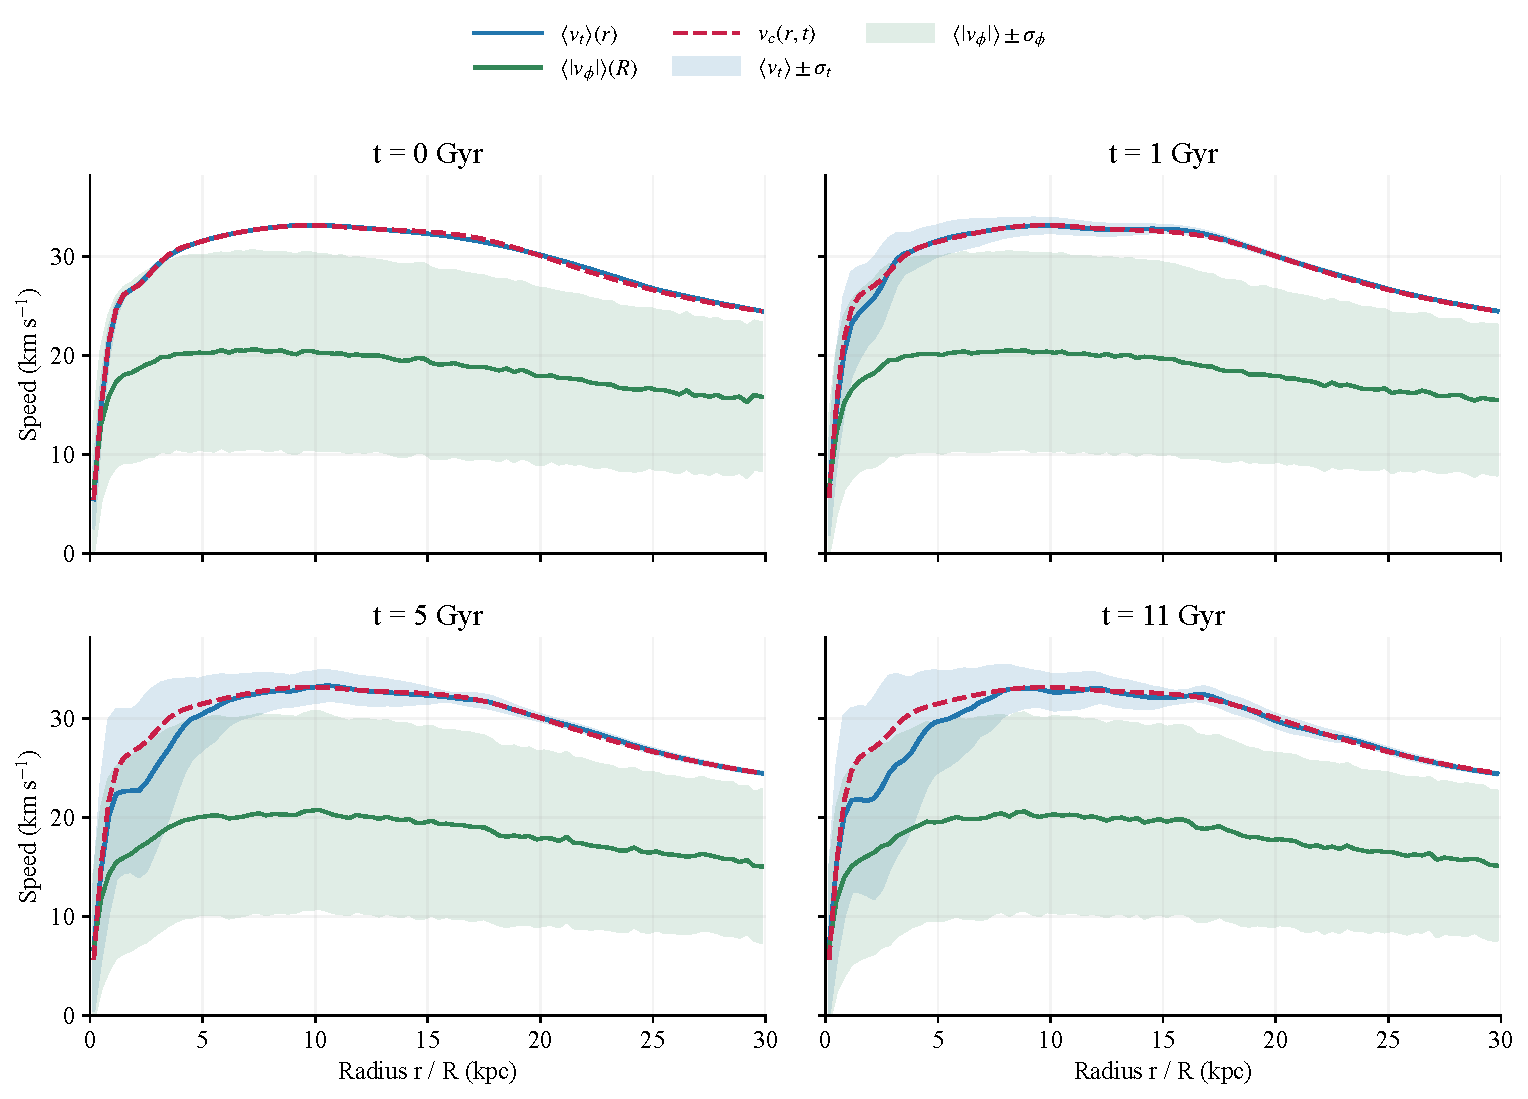
\includegraphics[width=\linewidth]{rotation_F3_M1e10_f0.0_four_epochs.pdf}
\caption{F3. Blue solid: $\vtmean(r,t)$. Green solid: $\langle|v_\phi|\rangle(R,t)$. Red dashed: $v_c(r,t)$. Blue and green bands: the corresponding mean $\pm1\sigma$. The green curve uses cylindrical $R$; the others use spherical $r$. The potential and red dashed reference are held fixed from 1 Gyr onward.}\label{fig:F3}
\end{figure}
\textbf{Animation:} \href{run:mp4/F3_M1e10_f0.0_frozen1Gyr.mp4}{View the F3 MP4 animation.}

The circular-speed reference is fixed after the ramp, and the late intermediate-radius stellar profile remains close to it. Compared with E3, the final speed ratio is closer to unity. The inner bins retain a finite dispersion and local offsets, even though the intermediate-radius median agrees well with the spherical reference.

For $B(t)=\operatorname{median}_{5\leq r/\mathrm{kpc}\leq20}[\vtmean/v_c]$, the four panels give $1.000$, $1.000$, $0.996$, $0.994$, respectively.
At 11 Gyr and $r=10\,\mathrm{kpc}$, $\vtmean=32.70\,\mathrm{km\,s^{-1}}$ and $v_c=33.16\,\mathrm{km\,s^{-1}}$.

\clearpage
\subsection{\texorpdfstring{F4: $M=10^{10}\,\Msun$, $f=0.1$, frozen at 1 Gyr}{F4: M=1e10 solar masses, f=0.1, frozen at 1 Gyr}}
\begin{figure}[!ht]
\centering
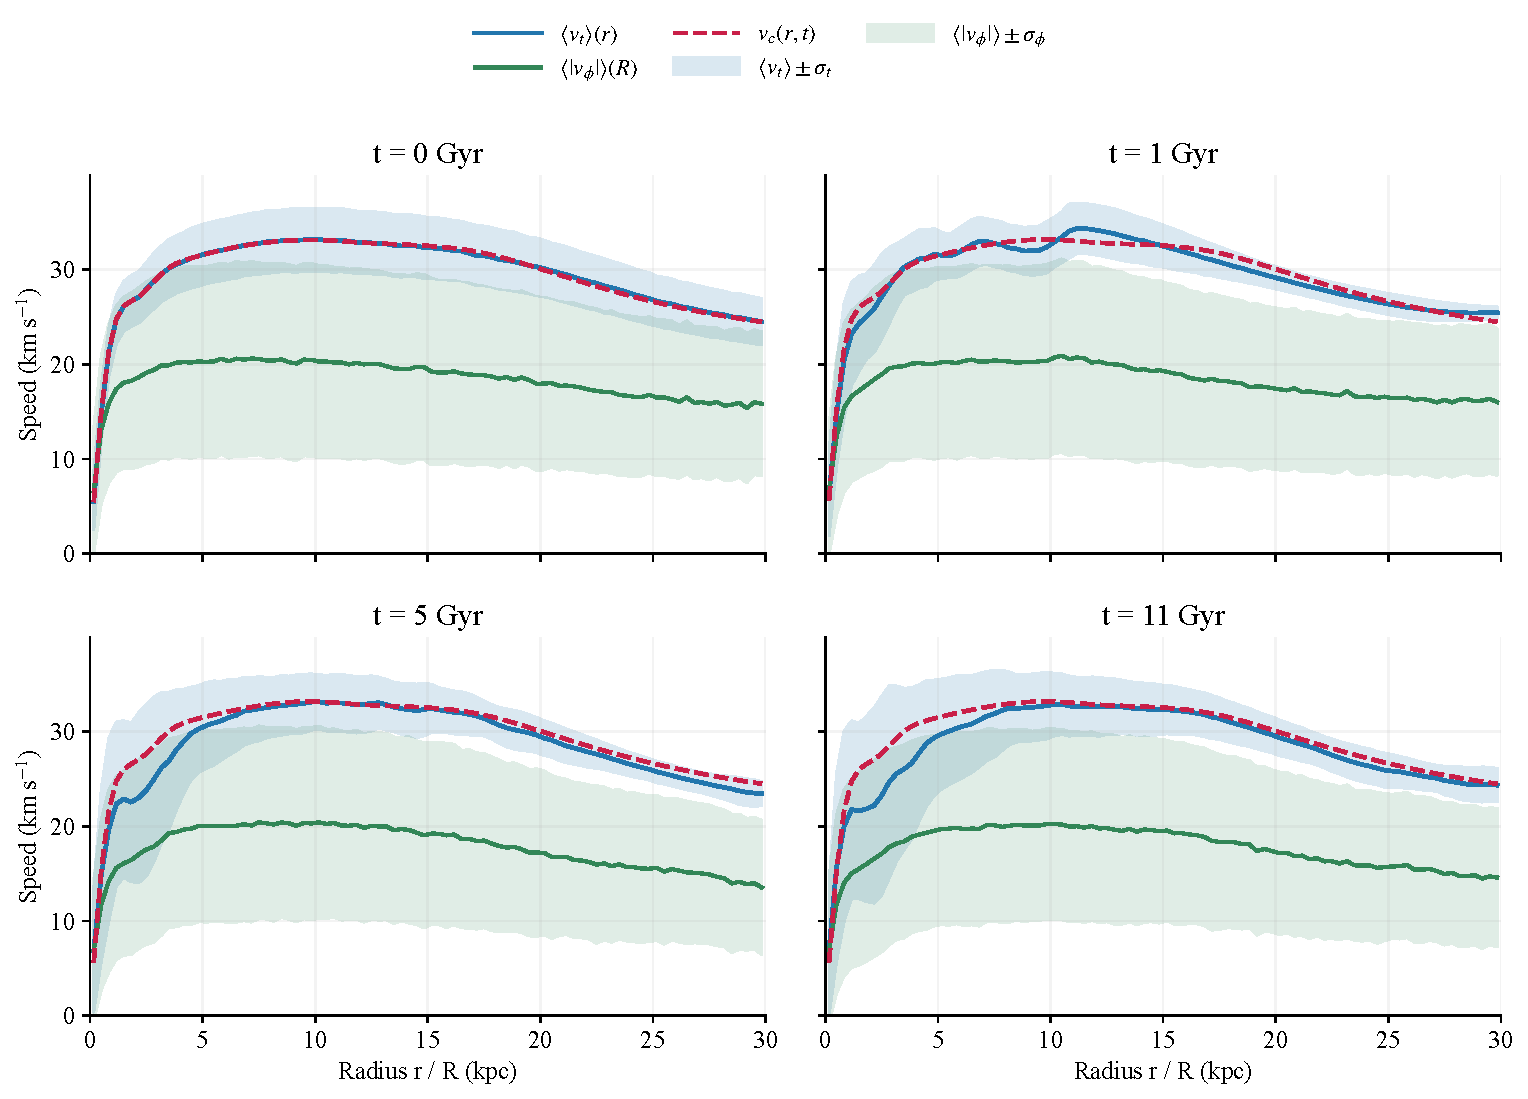
\includegraphics[width=\linewidth]{rotation_F4_M1e10_f0.1_four_epochs.pdf}
\caption{F4. Blue solid: $\vtmean(r,t)$. Green solid: $\langle|v_\phi|\rangle(R,t)$. Red dashed: $v_c(r,t)$. Blue and green bands: the corresponding mean $\pm1\sigma$. The green curve uses cylindrical $R$; the others use spherical $r$. The potential and red dashed reference are held fixed from 1 Gyr onward.}\label{fig:F4}
\end{figure}
\textbf{Animation:} \href{run:mp4/F4_M1e10_f0.1_frozen1Gyr.mp4}{View the F4 MP4 animation.}

The finite initial speed scatter broadens the first panel. After freezing, the late intermediate-radius mean remains close to the fixed reference, with a final median speed ratio similar to F3. Local differences and the particle-speed dispersion remain visible; a median ratio near unity does not imply equality of the curves at every radius.

For $B(t)=\operatorname{median}_{5\leq r/\mathrm{kpc}\leq20}[\vtmean/v_c]$, the four panels give $1.000$, $0.992$, $0.992$, $0.988$, respectively.
At 11 Gyr and $r=10\,\mathrm{kpc}$, $\vtmean=32.78\,\mathrm{km\,s^{-1}}$ and $v_c=33.16\,\mathrm{km\,s^{-1}}$.

\clearpage
\subsection{Comparison of the eight evolutions}
The same intermediate-radius statistic summarizes all eight figures:
\begin{equation}
 B(t)=\operatorname{median}_{j:\,5\leq r_j/\mathrm{kpc}\leq20}
       \left[\frac{\vtmean_j(t)}{v_c(r_j,t)}\right].
\end{equation}
This is an unweighted median over radial bins, not a particle-weighted
global mean. The reference is evaluated at the same plotted radius and
epoch as the tangential profile.

\begin{center}\small
\begin{tabular}{@{}ccrrrrr@{}}
\toprule
Run & History & $B(0)$ & $B(1)$ & $B(5)$ & $B(11)$ &
$\vtmean/v_c$ at 10 kpc, 11 Gyr\\
\midrule
E1 & Evolving & 1.000 & 1.001 & 0.840 & 0.846 & 0.756\\
E2 & Evolving & 1.000 & 0.993 & 0.840 & 0.844 & 0.768\\
E3 & Evolving & 1.000 & 1.000 & 0.974 & 0.938 & 0.931\\
E4 & Evolving & 1.000 & 0.992 & 0.977 & 0.939 & 0.924\\
F1 & Frozen & 1.000 & 1.001 & 0.953 & 0.965 & 0.947\\
F2 & Frozen & 1.000 & 0.993 & 0.944 & 0.968 & 0.947\\
F3 & Frozen & 1.000 & 1.000 & 0.996 & 0.994 & 0.986\\
F4 & Frozen & 1.000 & 0.992 & 0.992 & 0.988 & 0.989\\
\bottomrule
\end{tabular}
\end{center}

\textbf{Continuously evolving potentials.}
At 11 Gyr, $B\simeq0.844$--$0.846$ for $10^9\,\Msun$ and
$0.938$--$0.939$ for $10^{10}\,\Msun$. The intermediate-radius
mean tangential speed therefore falls below the spherical reference by
about 15\% and 6\%, respectively. The result is similar for $f=0$ and
$0.1$ within each halo model. The 5 and 11 Gyr panels also show that
the lower-mass median changes little over those epochs, whereas the
higher-mass median continues to decrease.

\textbf{Potentials frozen at 1 Gyr.}
At 11 Gyr the corresponding medians are $0.965$--$0.968$ and
$0.988$--$0.994$. Their intermediate-radius mean profiles lie closer to
the reference, while central offsets and nonzero dispersions persist.
The unchanged reference curves in the last three panels make clear that
the post-freeze changes arise from the continued evolution of the tracers
in the fixed field.

\textbf{Meaning of the measured offset.}
The figures compare a mean particle tangential-speed magnitude with an
enclosed-mass circular-speed reference. A population containing radial
motion and particles at different orbital phases need not satisfy
$\vtmean(r)=v_c(r)$. Likewise, the lower green curve in E1--E4 is an
absolute component-speed statistic and does not establish net rotation.
The evolving and frozen archives also use different coordinate
conventions, as stated in Section 1, so their numerical difference is
descriptive and does not isolate the effect of time-dependent forcing.
The eight figures establish the profile evolution and the residual
offsets for these stored experiments.
\end{document}
